\anonsection{Задание 1}

\anonsubsection{Формулировка задания}

\begin{enumerate}
	\item Реализовать генератор схемы Бернулли с заданной вероятностью
     успеха $p$. На основе генератора схемы Бернулли построить датчик
     для биномиального распределения.
	\item Реализовать генератор геометрического распределения. Проверить
     для данного распределения свойство отсутствия памяти.
	\item Рассмотреть игру в орлянку - бесконечную последеовательность
     независимых испытаний с бросанием правильной монеты.
     Выигрыш $S_n$ определяется как сумма по всем $n$ испытаниями 1 и -1
     в зависимости от выпавшей стороны. Проиллюстрировать (в виде ломанной)
     поведение нормированной суммы $Y(i) = S_i / \sqrt{n},$ как функцию
     от номера испытания $i = 1, \dots, n$ для одной отдельно взятой
     траектории. Дать теоритическую оценку для $Y(n)$
     при $n \longrightarrow \infty$.
\end{enumerate}

\anonsubsection{Генератор схемы Бернулли и биномиального распределения}
\begin{definition}
	Схемой Бернулли называется эксперимент, в котором проводится,
     вообще говоря, неограниченное количество испытаний. При этом каждому
     испытанию присваивается бинарный признак (успех --- $1$ или неудача --- $0$), и
     выполняются следующие требования:
	\begin{enumerate}
		\item отсутствие взаимного влияния;
		\item воспроизводимость;
		\item испытания проводятся в сходных условиях.
	\end{enumerate}
\end{definition}

\begin{definition}
	Случайная величина $X$, принимающая значение $1$ с вероятностью
     $p$ и значение $0$ с вероятностью $q = 1 - p$, называется случайной величиной
     с распределением Бернулли(или бернуллиевской случайной величиной).
\end{definition}

Для генератора схемы Бернулли реализуем генератор бернуллиевской случайной
 величины $X$. Для этого воспользуемся встроенным в библиотеку Numpy
 языка Python генератором равномерного распределения. Пусть тогда имеем
 случайную величину $Y \sim \Uni([0,1])$. В таком случае $X$
 можно представить в виде: $X = \Ind(Y < p)$, где $\Ind()$
 --- индикаторная функция:
$$
    X = \Ind(Y < p) = 
    \begin{cases}
        1 \ , & Y < p, \\
        0 \ , & Y \ge p.
    \end{cases}
$$
Генерация схемы Бернулли в таком случае будет происходить с помощью некоторого
 количества генераций бернуллиевской случайной величины.

\begin{definition}
	Случайная величина $X$ имеет биномиальное распределение с параметрами
     $n$ и $p$ $(X \sim \Bin(n,p))$, если
	$$ \mathbb{P}(X = k) = C^k_n p^k (1 - p)^{n - k}, \quad k \in
     \mathbb{N} \cup \{0\}. $$
\end{definition}

Случайную величину $X$ обычно интерпретируют как число успехов в схеме
 из $n$ испытаний Бернулли с вероятностью успеха $p$ в каждом. Поэтому
$$ X = \sum_{i = 1}^n Y_i ,$$
 где $Y_i \sim \Bern(p) \ , \ i = 1,\dots,n.$

 Промоделируем биномиальное распределение с параметрами $n = 50$, $p = 0.3$
 с помощью генерации схемы Бернулли с $n$ испытаниями:
 
 \begin{figure}[h]
	\begin{center}
		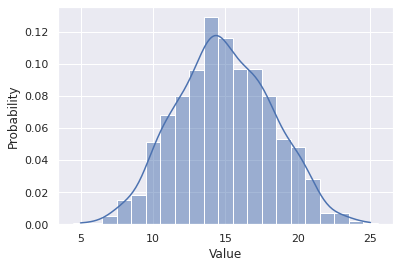
\includegraphics[width=0.85\linewidth]{"./resources/binominal.png"}
		\caption{Гистограмма биномиального распределения с $p = 0.3$, $n = 50$.}
          \label{fig:bin_dist}
	\end{center}
\end{figure}

\anonsubsection{Геометрическое распределение}

\begin{definition}
	Случайная величина $X$ имеет геометрическое распределение с
      параметром $p$ $(X\sim \Geom(p))$, если
	$$ \mathbb{P}(X = k) = (1 - p)^kp = q^k p \ , \ k \in \mathbb{N} \cup 
     \{0\}. $$
\end{definition}

Так же, как и в случае биномиального распределения, проводится некоторое
 количество испытаний Бернулли с одинаковой вероятностью успеха, до
 первого успеха. В качестве случайной величины с геометрическим распределением
 берется, как правило, количество неудач до первого успеха.

\anonsubsection{Свойство отсутствия памяти}
Случайная величина с геометрическим распределением обладает так называемым
 свойством отсутствия памяти. Неформально оно означает, что в момент проведения
 очередного испытания Бернулли количество прошлых неудач не влияет на количество
 будущих. Формально же это свойство можно сформулировать как
\newtheorem{stat}{Утверждение}
\begin{statement}
	Пусть $Y \sim \Geom(p)$, тогда $\forall m,n \in \mathbb{N} \cup 
     \{0\}$ справедливо:
	$$ 
     \mathbb{P}(Y > m + n \mid Y \ge m) = \mathbb{P}(Y > n),
     $$
\end{statement}
\begin{proof} Рассмотрим левую часть равенства:
     \begin{multline*}
          \mathbb{P}(Y > m + n \mid Y \ge m) = \dfrac{\mathbb{P}
          (Y > m + n, Y \ge m)}{\mathbb{P}(Y \ge m)} = \\
          = \dfrac{\mathbb{P}(Y > m + n)}{\mathbb{P}(Y \ge m)} = 
          \dfrac{\displaystyle\sum_{i = m + n + 1}^\infty q^i p}
          {\displaystyle\sum_{i = m}^\infty q^i p} = \dfrac{q^{m + n + 1}}{q^m} =
          q^{n + 1}.
     \end{multline*}
     С другой стороны, правая часть равна:
     $$ 
     \mathbb{P}(Y > n) = \sum_{i = n + 1}^\infty q^i p = p \dfrac{q^{n + 1}}
     {1 - q} = q^{n + 1}.
     $$
\end{proof}

Для демонстрации этого свойства в Python сгенерируем массив некоторого
 достаточного количества геометрических случаных величин. С помощью него
 построим гистограмму геометрического распределения (Рис. \eqref{subfig:geometric_distribution}). Зафиксируем некоторое $m$,
 и построим гистаграмму распределения вектора геометрических случайных
 величин из первоначального набора, значения которых больше либо равны $m$.
 В результате увидим, что при достаточно большом количестве чисел в первоначальном
 наборе гистограммы двух распределений приблизительно совпадают (Рис. \eqref{subfig:memoryless}). 

 \begin{figure}
     \centering
     \begin{subfigure}[b]{0.45\textwidth}
         \centering
         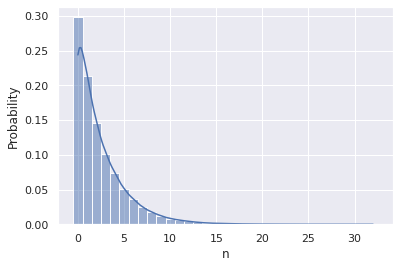
\includegraphics[width=\textwidth]{./resources/geometric.png}
         \caption{Гистограмма геометрического распределения при $p = 0.3$}
         \label{subfig:geometric_distribution}
     \end{subfigure}
     \hfill
     \begin{subfigure}[b]{0.45\textwidth}
         \centering
         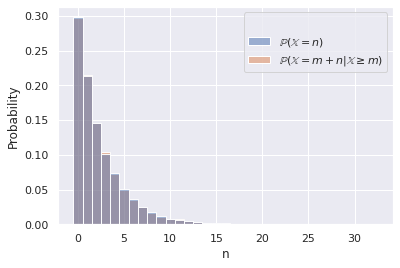
\includegraphics[width=\textwidth]{./resources/comparison.png}
         \caption{Демонстрация свойства отсутствия памяти}
         \label{subfig:memoryless}
     \end{subfigure}
     \caption{}
     \label{fig:geometric}
\end{figure}

\anonsubsection{Игра в орлянку}
Рассмотрим игру в орлянку. Для этого смоделируем последовательность
 случайных величин $X_1, X_2, \dots,$ где
$$
	X_i = 
	\begin{cases}
	     1 \ , & p = \frac{1}{2}\\
	     -1 \ , & p = \frac{1}{2}
	\end{cases}
     ,\quad i = 1,\dots,n.
$$
Тогда необходимая сумма представляется в виде:
$$
Y(i) = \dfrac{X_1 + \dots + X_i}{\sqrt n}, \quad
 i = 1,\dots,n ,
$$
где $n$ --- общее число генераций.

\begin{figure}[h]
	\begin{center}
		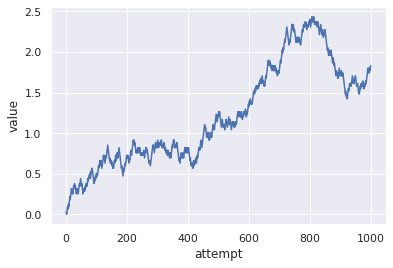
\includegraphics[width=0.75\linewidth]{"./resources/toss_game.png"}
		\caption{Траектория суммы $Y$ с $n = 1000$.}
	\end{center}
\end{figure}

Оценим $Y(n)$ при $n \to \infty$. Для этого сформулируем необходимую
 теорему.
\begin{theorem}[Центральная предельная теорема]
     Пусть $X_1,\dots, X_n,\dots$ есть бесконечная
      последовательность независимых одинаково распределенных случайных
      величин, имеющих конечное математическое ожидание $\mu$ и
      диспрерсию $\sigma^2$. Пусть также
     $$
     S_n = \displaystyle\sum_{i = 1}^n X_i
     $$
     Тогда
     $$
     \dfrac{S_n - \mu n}{\sigma \sqrt{n}} \to \Norm(0,1)
     $$
     по распределению при $n \to \infty$,
     где $\Norm(0,1)$ --- нормальное распределение с нулевым математическим ожиданием
      и стандартным отклонением, равным единице.
\end{theorem}

В случае игры Орлянки:
$$
\mu = \Exp[X_i] = 0, \quad
\sigma^2 = \Exp[(X_i - \Exp[X_i])^2] = 1, \quad i = 1, \dots, n
$$
Тогда поолучим, что последовательность случайных величин
$$
Y_n = Y(n) = \dfrac{S_n}{\sqrt{n}}
$$
Удовлетворяет условиям теоремы 1. Таким образом получаем, что $Y(n) \to \Norm(0,1)$.